\pgfdeclareplotmark{cross} {
\pgfpathmoveto{\pgfpoint{-0.3\pgfplotmarksize}{\pgfplotmarksize}}
\pgfpathlineto{\pgfpoint{+0.3\pgfplotmarksize}{\pgfplotmarksize}}
\pgfpathlineto{\pgfpoint{+0.3\pgfplotmarksize}{0.3\pgfplotmarksize}}
\pgfpathlineto{\pgfpoint{+1\pgfplotmarksize}{0.3\pgfplotmarksize}}
\pgfpathlineto{\pgfpoint{+1\pgfplotmarksize}{-0.3\pgfplotmarksize}}
\pgfpathlineto{\pgfpoint{+0.3\pgfplotmarksize}{-0.3\pgfplotmarksize}}
\pgfpathlineto{\pgfpoint{+0.3\pgfplotmarksize}{-1.\pgfplotmarksize}}
\pgfpathlineto{\pgfpoint{-0.3\pgfplotmarksize}{-1.\pgfplotmarksize}}
\pgfpathlineto{\pgfpoint{-0.3\pgfplotmarksize}{-0.3\pgfplotmarksize}}
\pgfpathlineto{\pgfpoint{-1.\pgfplotmarksize}{-0.3\pgfplotmarksize}}
\pgfpathlineto{\pgfpoint{-1.\pgfplotmarksize}{0.3\pgfplotmarksize}}
\pgfpathlineto{\pgfpoint{-0.3\pgfplotmarksize}{0.3\pgfplotmarksize}}
\pgfpathclose
\pgfusepathqstroke
}
\pgfdeclareplotmark{cross*} {
\pgfpathmoveto{\pgfpoint{-0.3\pgfplotmarksize}{\pgfplotmarksize}}
\pgfpathlineto{\pgfpoint{+0.3\pgfplotmarksize}{\pgfplotmarksize}}
\pgfpathlineto{\pgfpoint{+0.3\pgfplotmarksize}{0.3\pgfplotmarksize}}
\pgfpathlineto{\pgfpoint{+1\pgfplotmarksize}{0.3\pgfplotmarksize}}
\pgfpathlineto{\pgfpoint{+1\pgfplotmarksize}{-0.3\pgfplotmarksize}}
\pgfpathlineto{\pgfpoint{+0.3\pgfplotmarksize}{-0.3\pgfplotmarksize}}
\pgfpathlineto{\pgfpoint{+0.3\pgfplotmarksize}{-1.\pgfplotmarksize}}
\pgfpathlineto{\pgfpoint{-0.3\pgfplotmarksize}{-1.\pgfplotmarksize}}
\pgfpathlineto{\pgfpoint{-0.3\pgfplotmarksize}{-0.3\pgfplotmarksize}}
\pgfpathlineto{\pgfpoint{-1.\pgfplotmarksize}{-0.3\pgfplotmarksize}}
\pgfpathlineto{\pgfpoint{-1.\pgfplotmarksize}{0.3\pgfplotmarksize}}
\pgfpathlineto{\pgfpoint{-0.3\pgfplotmarksize}{0.3\pgfplotmarksize}}
\pgfpathclose
\pgfusepathqfillstroke
}
\pgfdeclareplotmark{newstar} {
\pgfpathmoveto{\pgfqpoint{0pt}{\pgfplotmarksize}}
\pgfpathlineto{\pgfqpointpolar{44}{0.5\pgfplotmarksize}}
\pgfpathlineto{\pgfqpointpolar{18}{\pgfplotmarksize}}
\pgfpathlineto{\pgfqpointpolar{-20}{0.5\pgfplotmarksize}}
\pgfpathlineto{\pgfqpointpolar{-54}{\pgfplotmarksize}}
\pgfpathlineto{\pgfqpointpolar{-90}{0.5\pgfplotmarksize}}
\pgfpathlineto{\pgfqpointpolar{234}{\pgfplotmarksize}}
\pgfpathlineto{\pgfqpointpolar{198}{0.5\pgfplotmarksize}}
\pgfpathlineto{\pgfqpointpolar{162}{\pgfplotmarksize}}
\pgfpathlineto{\pgfqpointpolar{134}{0.5\pgfplotmarksize}}
\pgfpathclose
\pgfusepathqstroke
}
\pgfdeclareplotmark{newstar*} {
\pgfpathmoveto{\pgfqpoint{0pt}{\pgfplotmarksize}}
\pgfpathlineto{\pgfqpointpolar{44}{0.5\pgfplotmarksize}}
\pgfpathlineto{\pgfqpointpolar{18}{\pgfplotmarksize}}
\pgfpathlineto{\pgfqpointpolar{-20}{0.5\pgfplotmarksize}}
\pgfpathlineto{\pgfqpointpolar{-54}{\pgfplotmarksize}}
\pgfpathlineto{\pgfqpointpolar{-90}{0.5\pgfplotmarksize}}
\pgfpathlineto{\pgfqpointpolar{234}{\pgfplotmarksize}}
\pgfpathlineto{\pgfqpointpolar{198}{0.5\pgfplotmarksize}}
\pgfpathlineto{\pgfqpointpolar{162}{\pgfplotmarksize}}
\pgfpathlineto{\pgfqpointpolar{134}{0.5\pgfplotmarksize}}
\pgfpathclose
\pgfusepathqfillstroke
}
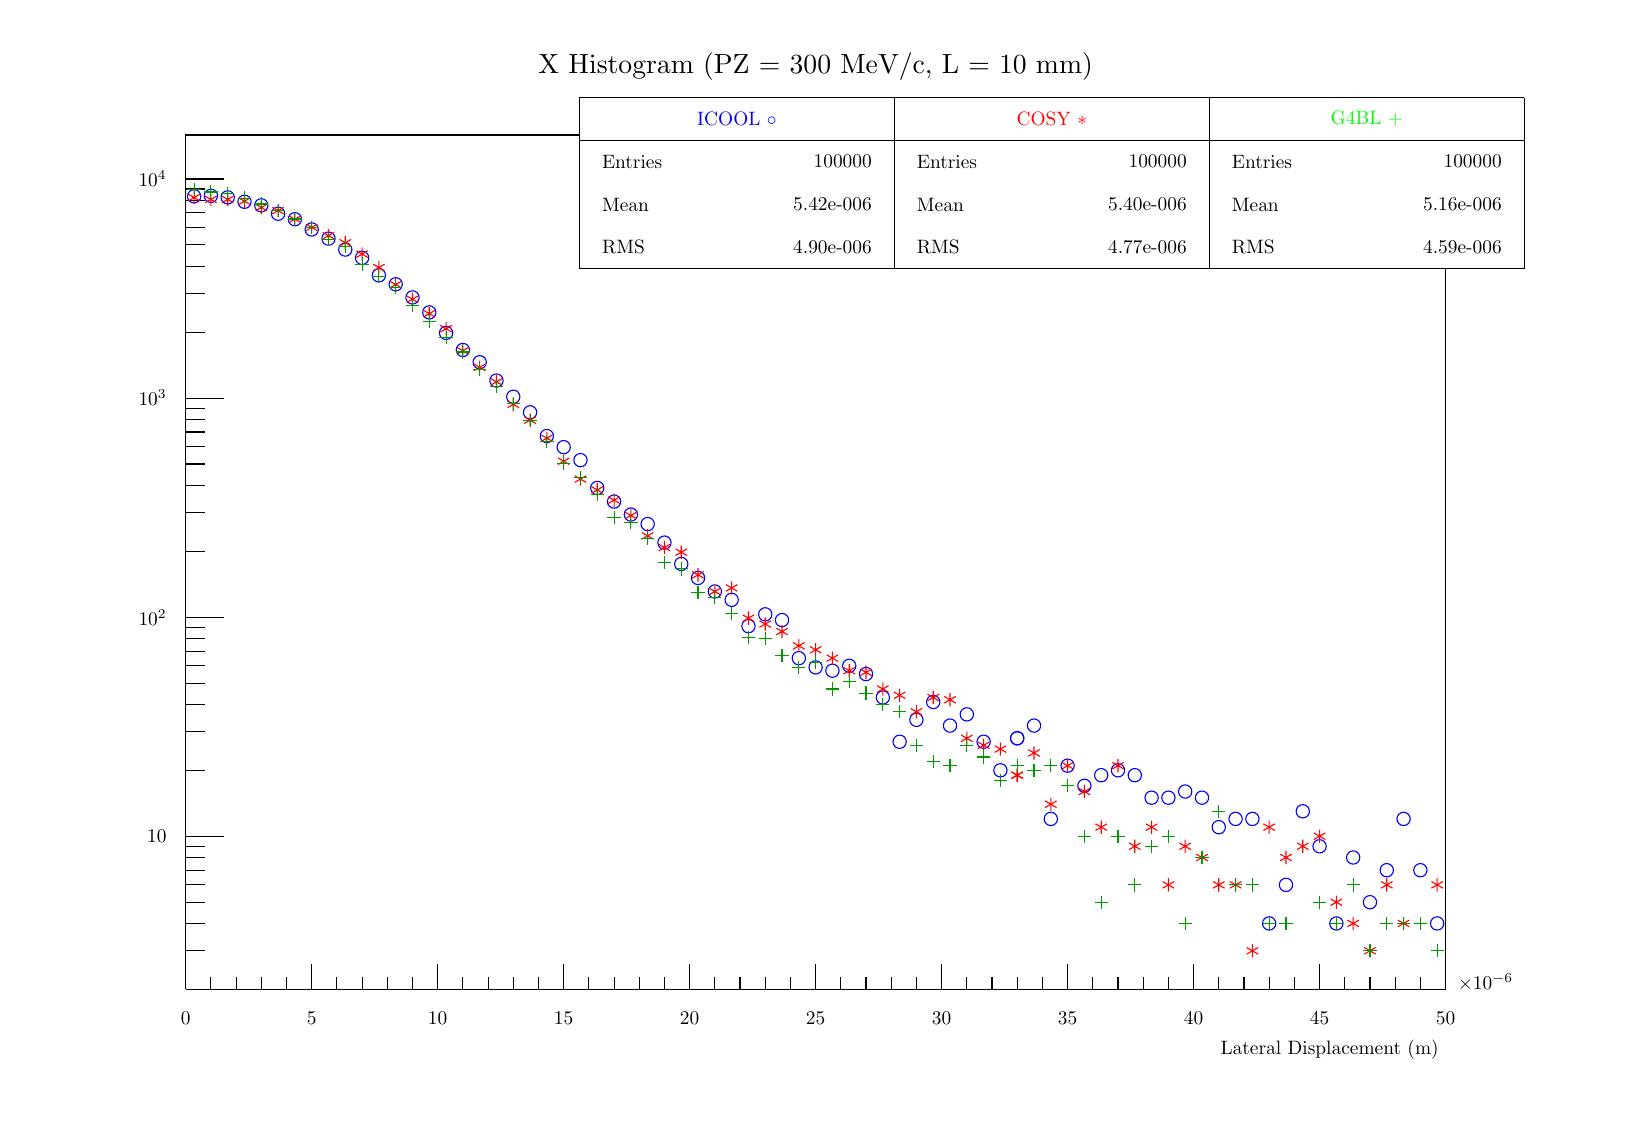
\begin{tikzpicture}
\definecolor{c}{rgb}{1,1,1};
\draw [color=c, fill=c] (0,0) rectangle (20,13.5632);
\draw [color=c, fill=c] (2,1.35632) rectangle (18,12.2069);
\definecolor{c}{rgb}{0,0,0};
\draw [c] (2,1.35632) -- (2,12.2069) -- (18,12.2069) -- (18,1.35632) -- (2,1.35632);
\definecolor{c}{rgb}{1,1,1};
\draw [color=c, fill=c] (2,1.35632) rectangle (18,12.2069);
\definecolor{c}{rgb}{0,0,0};
\draw [c] (2,1.35632) -- (2,12.2069) -- (18,12.2069) -- (18,1.35632) -- (2,1.35632);
\definecolor{c}{rgb}{0,0,1};
\foreach \P in
 {(2.10667,11.4283),(2.32,11.4346),(2.53333,11.415),(2.74667,11.3591),(2.96,11.3142),(3.17333,11.2073),(3.38667,11.1376),(3.6,11.0073),(3.81333,10.8909),(4.02667,10.7523),(4.24,10.6469),(4.45333,10.4248),(4.66667,10.3112),(4.88,10.1442),(5.09333,9.95
418),(5.30667,9.69383),(5.52,9.47692),(5.73333,9.32076),(5.94667,9.08827),(6.16,8.88275),(6.37333,8.6851),(6.58667,8.38382),(6.8,8.24262),(7.01333,8.07808),(7.22667,7.72502),(7.44,7.55162),(7.65333,7.38668),(7.86667,7.26574),(8.08,7.0308),(8.29333,6.
75977),(8.50667,6.58153),(8.72,6.40984),(8.93333,6.30386),(9.14667,5.96958),(9.36,6.11926),(9.57333,6.04674),(9.78667,5.56299),(10,5.44596),(10.2133,5.40429),(10.4267,5.46627),(10.64,5.36113),(10.8533,5.0637),(11.0667,4.50137),(11.28,4.77993),(11.493
3,5.00615),(11.7067,4.70667),(11.92,4.849),(12.1333,4.50137),(12.3467,4.13873),(12.56,4.54531)}{\draw[mark options={color=c,fill=c},mark size=2.402402pt,mark=o] plot coordinates {\P};}
\foreach \P in
 {(12.56,4.54531),(12.7733,4.70667),(12.9867,3.52145),(13.2,4.19768),(13.4133,3.94234),(13.6267,4.07674),(13.84,4.13873),(14.0533,4.07674),(14.2667,3.7911),(14.48,3.7911),(14.6933,3.86908),(14.9067,3.7911),(15.12,3.41631),(15.3333,3.52145),(15.5467,3
.52145),(15.76,2.19391),(15.9733,2.68387),(16.1867,3.61818),(16.4,3.17382),(16.6133,2.19391),(16.8267,3.0315),(17.04,2.46355),(17.2533,2.87014),(17.4667,3.52145),(17.68,2.87014),(17.8933,2.19391)}{\draw[mark options={color=c,fill=c},mark
 size=2.402402pt,mark=o] plot coordinates {\P};}
\definecolor{c}{rgb}{1,1,1};
\draw [color=c, fill=c] (7,10.5115) rectangle (11,12.6816);
\definecolor{c}{rgb}{0,0,0};
\draw [c] (7,10.5115) -- (11,10.5115);
\draw [c] (11,10.5115) -- (11,12.6816);
\draw [c] (11,12.6816) -- (7,12.6816);
\draw [c] (7,12.6816) -- (7,10.5115);
\draw[color=blue](9,12.4103) node[scale=0.7, rotate=0]{ICOOL $\circ$};
\draw [c] (7,12.1391) -- (11,12.1391);
\draw [anchor= west] (7.2,11.8678) node[scale=0.7, rotate=0]{Entries };
\draw [anchor= east] (10.8,11.8678) node[scale=0.7, rotate=0]{ 100000};
\draw [anchor= west] (7.2,11.3253) node[scale=0.7, rotate=0]{Mean  };
\draw [anchor= east] (10.8,11.3253) node[scale=0.7, rotate=0]{ 5.42e-006};
\draw [anchor= west] (7.2,10.7828) node[scale=0.7, rotate=0]{RMS   };
\draw [anchor= east] (10.8,10.7828) node[scale=0.7, rotate=0]{ 4.90e-006};
\draw [c] (2,1.35632) -- (18,1.35632);
\draw [anchor= east] (18,0.596782) node[scale=0.7, rotate=0]{Lateral Displacement (m)};
\draw [c] (2,1.68184) -- (2,1.35632);
\draw [c] (2.32,1.51908) -- (2.32,1.35632);
\draw [c] (2.64,1.51908) -- (2.64,1.35632);
\draw [c] (2.96,1.51908) -- (2.96,1.35632);
\draw [c] (3.28,1.51908) -- (3.28,1.35632);
\draw [c] (3.6,1.68184) -- (3.6,1.35632);
\draw [c] (3.92,1.51908) -- (3.92,1.35632);
\draw [c] (4.24,1.51908) -- (4.24,1.35632);
\draw [c] (4.56,1.51908) -- (4.56,1.35632);
\draw [c] (4.88,1.51908) -- (4.88,1.35632);
\draw [c] (5.2,1.68184) -- (5.2,1.35632);
\draw [c] (5.52,1.51908) -- (5.52,1.35632);
\draw [c] (5.84,1.51908) -- (5.84,1.35632);
\draw [c] (6.16,1.51908) -- (6.16,1.35632);
\draw [c] (6.48,1.51908) -- (6.48,1.35632);
\draw [c] (6.8,1.68184) -- (6.8,1.35632);
\draw [c] (7.12,1.51908) -- (7.12,1.35632);
\draw [c] (7.44,1.51908) -- (7.44,1.35632);
\draw [c] (7.76,1.51908) -- (7.76,1.35632);
\draw [c] (8.08,1.51908) -- (8.08,1.35632);
\draw [c] (8.4,1.68184) -- (8.4,1.35632);
\draw [c] (8.72,1.51908) -- (8.72,1.35632);
\draw [c] (9.04,1.51908) -- (9.04,1.35632);
\draw [c] (9.36,1.51908) -- (9.36,1.35632);
\draw [c] (9.68,1.51908) -- (9.68,1.35632);
\draw [c] (10,1.68184) -- (10,1.35632);
\draw [c] (10.32,1.51908) -- (10.32,1.35632);
\draw [c] (10.64,1.51908) -- (10.64,1.35632);
\draw [c] (10.96,1.51908) -- (10.96,1.35632);
\draw [c] (11.28,1.51908) -- (11.28,1.35632);
\draw [c] (11.6,1.68184) -- (11.6,1.35632);
\draw [c] (11.92,1.51908) -- (11.92,1.35632);
\draw [c] (12.24,1.51908) -- (12.24,1.35632);
\draw [c] (12.56,1.51908) -- (12.56,1.35632);
\draw [c] (12.88,1.51908) -- (12.88,1.35632);
\draw [c] (13.2,1.68184) -- (13.2,1.35632);
\draw [c] (13.52,1.51908) -- (13.52,1.35632);
\draw [c] (13.84,1.51908) -- (13.84,1.35632);
\draw [c] (14.16,1.51908) -- (14.16,1.35632);
\draw [c] (14.48,1.51908) -- (14.48,1.35632);
\draw [c] (14.8,1.68184) -- (14.8,1.35632);
\draw [c] (15.12,1.51908) -- (15.12,1.35632);
\draw [c] (15.44,1.51908) -- (15.44,1.35632);
\draw [c] (15.76,1.51908) -- (15.76,1.35632);
\draw [c] (16.08,1.51908) -- (16.08,1.35632);
\draw [c] (16.4,1.68184) -- (16.4,1.35632);
\draw [c] (16.72,1.51908) -- (16.72,1.35632);
\draw [c] (17.04,1.51908) -- (17.04,1.35632);
\draw [c] (17.36,1.51908) -- (17.36,1.35632);
\draw [c] (17.68,1.51908) -- (17.68,1.35632);
\draw [c] (18,1.68184) -- (18,1.35632);
\draw [c] (18,1.68184) -- (18,1.35632);
\draw [anchor=base] (2,0.908736) node[scale=0.7, rotate=0]{0};
\draw [anchor=base] (3.6,0.908736) node[scale=0.7, rotate=0]{5};
\draw [anchor=base] (5.2,0.908736) node[scale=0.7, rotate=0]{10};
\draw [anchor=base] (6.8,0.908736) node[scale=0.7, rotate=0]{15};
\draw [anchor=base] (8.4,0.908736) node[scale=0.7, rotate=0]{20};
\draw [anchor=base] (10,0.908736) node[scale=0.7, rotate=0]{25};
\draw [anchor=base] (11.6,0.908736) node[scale=0.7, rotate=0]{30};
\draw [anchor=base] (13.2,0.908736) node[scale=0.7, rotate=0]{35};
\draw [anchor=base] (14.8,0.908736) node[scale=0.7, rotate=0]{40};
\draw [anchor=base] (16.4,0.908736) node[scale=0.7, rotate=0]{45};
\draw [anchor=base] (18,0.908736) node[scale=0.7, rotate=0]{50};
\draw [anchor=base west] (18.07,1.35632) node[scale=0.7, rotate=0]{$\times10^{-6}$};
\draw [c] (2,1.35632) -- (2,12.2069);
\draw [c] (2.24,1.84628) -- (2,1.84628);
\draw [c] (2.24,2.19391) -- (2,2.19391);
\draw [c] (2.24,2.46355) -- (2,2.46355);
\draw [c] (2.24,2.68386) -- (2,2.68386);
\draw [c] (2.24,2.87014) -- (2,2.87014);
\draw [c] (2.24,3.03149) -- (2,3.03149);
\draw [c] (2.24,3.17382) -- (2,3.17382);
\draw [c] (2.48,3.30114) -- (2,3.30114);
\draw [anchor= east] (1.844,3.30114) node[scale=0.7, rotate=0]{10};
\draw [c] (2.24,4.13872) -- (2,4.13872);
\draw [c] (2.24,4.62868) -- (2,4.62868);
\draw [c] (2.24,4.97631) -- (2,4.97631);
\draw [c] (2.24,5.24595) -- (2,5.24595);
\draw [c] (2.24,5.46627) -- (2,5.46627);
\draw [c] (2.24,5.65254) -- (2,5.65254);
\draw [c] (2.24,5.8139) -- (2,5.8139);
\draw [c] (2.24,5.95623) -- (2,5.95623);
\draw [c] (2.48,6.08354) -- (2,6.08354);
\draw [anchor= east] (1.844,6.08354) node[scale=0.7, rotate=0]{$10^{2}$};
\draw [c] (2.24,6.92113) -- (2,6.92113);
\draw [c] (2.24,7.41109) -- (2,7.41109);
\draw [c] (2.24,7.75872) -- (2,7.75872);
\draw [c] (2.24,8.02836) -- (2,8.02836);
\draw [c] (2.24,8.24867) -- (2,8.24867);
\draw [c] (2.24,8.43495) -- (2,8.43495);
\draw [c] (2.24,8.5963) -- (2,8.5963);
\draw [c] (2.24,8.73863) -- (2,8.73863);
\draw [c] (2.48,8.86595) -- (2,8.86595);
\draw [anchor= east] (1.844,8.86595) node[scale=0.7, rotate=0]{$10^{3}$};
\draw [c] (2.24,9.70354) -- (2,9.70354);
\draw [c] (2.24,10.1935) -- (2,10.1935);
\draw [c] (2.24,10.5411) -- (2,10.5411);
\draw [c] (2.24,10.8108) -- (2,10.8108);
\draw [c] (2.24,11.0311) -- (2,11.0311);
\draw [c] (2.24,11.2174) -- (2,11.2174);
\draw [c] (2.24,11.3787) -- (2,11.3787);
\draw [c] (2.24,11.521) -- (2,11.521);
\draw [c] (2.48,11.6484) -- (2,11.6484);
\draw [anchor= east] (1.844,11.6484) node[scale=0.7, rotate=0]{$10^{4}$};
\definecolor{c}{rgb}{1,1,1};
\draw [color=c, fill=c] (7,10.5115) rectangle (11,12.6816);
\definecolor{c}{rgb}{0,0,0};
\draw [c] (7,10.5115) -- (11,10.5115);
\draw [c] (11,10.5115) -- (11,12.6816);
\draw [c] (11,12.6816) -- (7,12.6816);
\draw [c] (7,12.6816) -- (7,10.5115);
\draw[color=blue](9,12.4103) node[scale=0.7, rotate=0]{ICOOL $\circ$};
\draw [c] (7,12.1391) -- (11,12.1391);
\draw [anchor= west] (7.2,11.8678) node[scale=0.7, rotate=0]{Entries };
\draw [anchor= east] (10.8,11.8678) node[scale=0.7, rotate=0]{ 100000};
\draw [anchor= west] (7.2,11.3253) node[scale=0.7, rotate=0]{Mean  };
\draw [anchor= east] (10.8,11.3253) node[scale=0.7, rotate=0]{ 5.42e-006};
\draw [anchor= west] (7.2,10.7828) node[scale=0.7, rotate=0]{RMS   };
\draw [anchor= east] (10.8,10.7828) node[scale=0.7, rotate=0]{ 4.90e-006};
\draw (10,13.0816) node[scale=1, rotate=0]{X Histogram (PZ = 300 MeV/c, L = 10 mm)};
\definecolor{c}{rgb}{1,0,0};
\foreach \P in
 {(2.10667,11.4127),(2.32,11.3891),(2.53333,11.3888),(2.74667,11.3663),(2.96,11.2863),(3.17333,11.246),(3.38667,11.1372),(3.6,11.0335),(3.81333,10.9284),(4.02667,10.839),(4.24,10.6944),(4.45333,10.5241),(4.66667,10.3079),(4.88,10.1213),(5.09333,9.937
87),(5.30667,9.74744),(5.52,9.46667),(5.73333,9.25602),(5.94667,9.07208),(6.16,8.78603),(6.37333,8.58569),(6.58667,8.3565),(6.8,8.06408),(7.01333,7.83765),(7.22667,7.69991),(7.44,7.56942),(7.65333,7.37428),(7.86667,7.116),(8.08,6.96852),(8.29333,6.90
899),(8.50667,6.62089),(8.72,6.40984),(8.93333,6.4551),(9.14667,6.0714),(9.36,5.99585),(9.57333,5.90129),(9.78667,5.71969),(10,5.66968),(10.2133,5.56299),(10.4267,5.40429),(10.64,5.3829),(10.8533,5.17119),(11.0667,5.09149),(11.28,4.88211),(11.4933,5.
0637),(11.7067,5.03527),(11.92,4.54531),(12.1333,4.45576),(12.3467,4.40837),(12.56,4.07674)}{\draw[mark options={color=c,fill=c},mark size=2.402402pt,mark=asterisk] plot coordinates {\P};}
\foreach \P in
 {(12.56,4.07674),(12.7733,4.35904),(12.9867,3.70773),(13.2,4.19768),(13.4133,3.86908),(13.6267,3.41631),(13.84,4.19768),(14.0533,3.17382),(14.2667,3.41631),(14.48,2.68387),(14.6933,3.17382),(14.9067,3.0315),(15.12,2.68387),(15.3333,2.68387),(15.5467
,1.84628),(15.76,3.41631),(15.9733,3.0315),(16.1867,3.17382),(16.4,3.30114),(16.6133,2.46355),(16.8267,2.19391),(17.04,1.84628),(17.2533,2.68387),(17.4667,2.19391),(17.8933,2.68387)}{\draw[mark options={color=c,fill=c},mark
 size=2.402402pt,mark=asterisk] plot coordinates {\P};}
\definecolor{c}{rgb}{1,1,1};
\draw [color=c, fill=c] (11,10.5115) rectangle (15,12.6816);
\definecolor{c}{rgb}{0,0,0};
\draw [c] (11,10.5115) -- (15,10.5115);
\draw [c] (15,10.5115) -- (15,12.6816);
\draw [c] (15,12.6816) -- (11,12.6816);
\draw [c] (11,12.6816) -- (11,10.5115);
\draw [color=red](13,12.4103) node[scale=0.7, rotate=0]{COSY $*$};
\draw [c] (11,12.1391) -- (15,12.1391);
\draw [anchor= west] (11.2,11.8678) node[scale=0.7, rotate=0]{Entries };
\draw [anchor= east] (14.8,11.8678) node[scale=0.7, rotate=0]{ 100000};
\draw [anchor= west] (11.2,11.3253) node[scale=0.7, rotate=0]{Mean  };
\draw [anchor= east] (14.8,11.3253) node[scale=0.7, rotate=0]{ 5.40e-006};
\draw [anchor= west] (11.2,10.7828) node[scale=0.7, rotate=0]{RMS   };
\draw [anchor= east] (14.8,10.7828) node[scale=0.7, rotate=0]{ 4.77e-006};
\definecolor{c}{rgb}{1,1,1};
\draw [color=c, fill=c] (11,10.5115) rectangle (15,12.6816);
\definecolor{c}{rgb}{0,0,0};
\draw [c] (11,10.5115) -- (15,10.5115);
\draw [c] (15,10.5115) -- (15,12.6816);
\draw [c] (15,12.6816) -- (11,12.6816);
\draw [c] (11,12.6816) -- (11,10.5115);
\draw [color=red](13,12.4103) node[scale=0.7, rotate=0]{COSY $*$};
\draw [c] (11,12.1391) -- (15,12.1391);
\draw [anchor= west] (11.2,11.8678) node[scale=0.7, rotate=0]{Entries };
\draw [anchor= east] (14.8,11.8678) node[scale=0.7, rotate=0]{ 100000};
\draw [anchor= west] (11.2,11.3253) node[scale=0.7, rotate=0]{Mean  };
\draw [anchor= east] (14.8,11.3253) node[scale=0.7, rotate=0]{ 5.40e-006};
\draw [anchor= west] (11.2,10.7828) node[scale=0.7, rotate=0]{RMS   };
\draw [anchor= east] (14.8,10.7828) node[scale=0.7, rotate=0]{ 4.77e-006};
\definecolor{c}{rgb}{0,0.6,0};
\foreach \P in
 {(2.10667,11.513),(2.32,11.4834),(2.53333,11.4639),(2.74667,11.4062),(2.96,11.3302),(3.17333,11.2469),(3.38667,11.1404),(3.6,11.0315),(3.81333,10.8823),(4.02667,10.7873),(4.24,10.5671),(4.45333,10.4094),(4.66667,10.2666),(4.88,10.0436),(5.09333,9.84
317),(5.30667,9.63773),(5.52,9.45114),(5.73333,9.22948),(5.94667,9.01363),(6.16,8.79759),(6.37333,8.58111),(6.58667,8.31337),(6.8,8.04039),(7.01333,7.85451),(7.22667,7.6381),(7.44,7.35334),(7.65333,7.28824),(7.86667,7.07946),(8.08,6.77351),(8.29333,6
.69597),(8.50667,6.40058),(8.72,6.3337),(8.93333,6.13094),(9.14667,5.82891),(9.36,5.8139),(9.57333,5.59961),(9.78667,5.44596),(10,5.50589),(10.2133,5.17119),(10.4267,5.26989),(10.64,5.11864),(10.8533,4.97631),(11.0667,4.88211),(11.28,4.45576),(11.493
3,4.2539),(11.7067,4.19768),(11.92,4.45576),(12.1333,4.30761),(12.3467,4.01141),(12.56,4.19768)}{\draw[mark options={color=c,fill=c},mark size=2.402402pt,mark=+] plot coordinates {\P};}
\foreach \P in
 {(12.56,4.19768),(12.7733,4.13873),(12.9867,4.19768),(13.2,3.94234),(13.4133,3.30114),(13.6267,2.46355),(13.84,3.30114),(14.0533,2.68387),(14.2667,3.17382),(14.48,3.30114),(14.6933,2.19391),(14.9067,3.0315),(15.12,3.61818),(15.3333,2.68387),(15.5467
,2.68387),(15.76,2.19391),(15.9733,2.19391),(16.4,2.46355),(16.6133,2.19391),(16.8267,2.68387),(17.04,1.84628),(17.2533,2.19391),(17.4667,2.19391),(17.68,2.19391),(17.8933,1.84628)}{\draw[mark options={color=c,fill=c},mark size=2.402402pt,mark=+]
 plot coordinates {\P};}
\definecolor{c}{rgb}{1,1,1};
\draw [color=c, fill=c] (15,10.5115) rectangle (19,12.6816);
\definecolor{c}{rgb}{0,0,0};
\draw [c] (15,10.5115) -- (19,10.5115);
\draw [c] (19,10.5115) -- (19,12.6816);
\draw [c] (19,12.6816) -- (15,12.6816);
\draw [c] (15,12.6816) -- (15,10.5115);
\draw [color=green](17,12.4103) node[scale=0.7, rotate=0]{G4BL $+$};
\draw [c] (15,12.1391) -- (19,12.1391);
\draw [anchor= west] (15.2,11.8678) node[scale=0.7, rotate=0]{Entries };
\draw [anchor= east] (18.8,11.8678) node[scale=0.7, rotate=0]{ 100000};
\draw [anchor= west] (15.2,11.3253) node[scale=0.7, rotate=0]{Mean  };
\draw [anchor= east] (18.8,11.3253) node[scale=0.7, rotate=0]{ 5.16e-006};
\draw [anchor= west] (15.2,10.7828) node[scale=0.7, rotate=0]{RMS   };
\draw [anchor= east] (18.8,10.7828) node[scale=0.7, rotate=0]{ 4.59e-006};
\definecolor{c}{rgb}{1,1,1};
\draw [color=c, fill=c] (15,10.5115) rectangle (19,12.6816);
\definecolor{c}{rgb}{0,0,0};
\draw [c] (15,10.5115) -- (19,10.5115);
\draw [c] (19,10.5115) -- (19,12.6816);
\draw [c] (19,12.6816) -- (15,12.6816);
\draw [c] (15,12.6816) -- (15,10.5115);
\draw [color=green](17,12.4103) node[scale=0.7, rotate=0]{G4BL $+$};
\draw [c] (15,12.1391) -- (19,12.1391);
\draw [anchor= west] (15.2,11.8678) node[scale=0.7, rotate=0]{Entries };
\draw [anchor= east] (18.8,11.8678) node[scale=0.7, rotate=0]{ 100000};
\draw [anchor= west] (15.2,11.3253) node[scale=0.7, rotate=0]{Mean  };
\draw [anchor= east] (18.8,11.3253) node[scale=0.7, rotate=0]{ 5.16e-006};
\draw [anchor= west] (15.2,10.7828) node[scale=0.7, rotate=0]{RMS   };
\draw [anchor= east] (18.8,10.7828) node[scale=0.7, rotate=0]{ 4.59e-006};
\end{tikzpicture}
